% ATLAS: technical guide -- every feature and how it is built, so the team can explain the work and answer questions.
% Written by hand; compile with pdflatex. The look follows the other ATLAS handouts. 4 October 2026.
\documentclass[10pt]{article}
\usepackage[a4paper,top=14mm,bottom=17mm,left=16mm,right=16mm,footskip=9mm]{geometry}
\usepackage[T1]{fontenc}
\usepackage[utf8]{inputenc}
\input{glyphtounicode}\pdfgentounicode=1
\usepackage{helvet}
\renewcommand{\familydefault}{\sfdefault}
\usepackage[varqu,varl]{zi4}
\usepackage{amsmath,amssymb}
\usepackage[helvet]{sfmath}
\usepackage[table]{xcolor}
\usepackage{array,booktabs,tabularx}
\usepackage{enumitem}
\usepackage{needspace}
\usepackage{tikz}
\usetikzlibrary{arrows.meta,positioning}

\pdfinfo{/Title (ATLAS: technical guide)}

% ---------- colours (the palette of the other ATLAS handouts) ----------
\definecolor{ink}{HTML}{1F2933}
\definecolor{mute}{HTML}{56616B}
\definecolor{laneD}{HTML}{E3EDFC}
\definecolor{accC}{HTML}{9A4A00}
\definecolor{accD}{HTML}{1B55B0}
\definecolor{cmdbg}{HTML}{F1F3F5}
\definecolor{trapbg}{HTML}{FDF3E7}

% ---------- footer ----------
\makeatletter
\def\ps@atlas{%
  \def\@oddhead{}\def\@evenhead{}%
  \def\@oddfoot{\parbox{\textwidth}{\footnotesize\color{mute}ATLAS: technical guide\hfill 4 October 2026\hspace{6mm}Page \thepage}}%
  \let\@evenfoot\@oddfoot}
\makeatother
\pagestyle{atlas}

\setlength{\parindent}{0pt}
\setlength{\parskip}{3pt}
\color{ink}
\setlist[itemize]{leftmargin=4.5mm,itemsep=1pt,topsep=1.5pt,parsep=0pt,partopsep=0pt}
\setlist[enumerate]{leftmargin=5.5mm,itemsep=1pt,topsep=1.5pt,parsep=0pt,partopsep=0pt}
\renewcommand{\arraystretch}{1.18}

% ---------- building blocks ----------
\newcounter{sec}
% \Sec{title}   a numbered part
\newcommand{\Sec}[1]{\Needspace{38mm}\refstepcounter{sec}\vspace{5mm}%
  \noindent{\color{accD}\rule{\textwidth}{0.9pt}}\par\vspace{1mm}%
  \noindent{\Large\bfseries{\color{accD}\thesec}\hspace{3mm}#1}\par\vspace{1.5mm}}
% \Sub{title}   a heading inside a part
\newcommand{\Sub}[1]{\Needspace{18mm}\vspace{2.5mm}\noindent{\bfseries\color{accD}#1}\par\vspace{0.3mm}}
% \Key{text}    the thing to remember
\newcommand{\Key}[1]{\par\vspace{1.5mm}\noindent{\setlength{\fboxsep}{3mm}\colorbox{laneD}{\parbox{\dimexpr\textwidth-6mm}{#1}}}\par\vspace{1.5mm}}
% \Status{text} what is proven and what is not
\newcommand{\Status}[1]{\par\vspace{1.5mm}\noindent{\setlength{\fboxsep}{2.2mm}\colorbox{trapbg}{\parbox{\dimexpr\textwidth-4.4mm}{\small\textbf{\color{accC}Status.} #1}}}\par}
% questions a judge may ask, with the answer
\newenvironment{asked}{\Needspace{16mm}\par\vspace{2mm}\noindent{\small\bfseries\color{accC}If asked}%
  \begin{itemize}[leftmargin=4.5mm,itemsep=1.5pt,topsep=1pt]\small}{\end{itemize}}
\newcommand{\Q}[1]{\item \textbf{#1}}
\newcommand{\code}[1]{{\ttfamily\fontsize{8.8}{11}\selectfont #1}}
\newcommand{\R}{\mathbb{R}}
\newcommand{\Hyp}{\mathbb{H}^2}
\newcommand{\Sph}{\mathbb{S}^2}

\begin{document}

% ====================================================================================================
{\fontsize{22}{26}\selectfont\bfseries ATLAS: technical guide}\par\vspace{1.5mm}
{\large\color{mute}Every feature and how it is built. Enough to explain the work and answer questions.}\par\vspace{1mm}
{\footnotesize\color{mute}4 October 2026. Taken from the code, the contract pages (\code{docs/contracts/}) and the Master Plan. Where this guide and the code differ, the code is right.}

% ====================================================================================================
\Sec{ATLAS on one page}

ATLAS is our entry for Huawei Custom Challenge 1, ``Beyond Euclid''. A phone in a lens headset scans your room; the room becomes the first tile of other universes, and you walk through them on your own feet.

\begin{center}
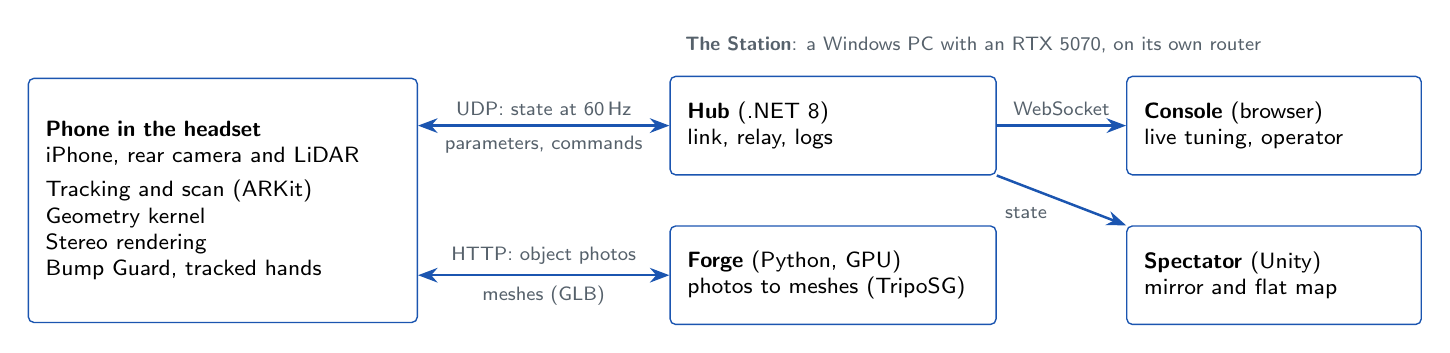
\begin{tikzpicture}[>=Stealth,
  box/.style={draw=accD,line width=0.5pt,rounded corners=2pt,inner sep=2.2mm,align=left,font=\footnotesize},
  lab/.style={font=\scriptsize,color=mute,align=center}]
\node[box,text width=45mm,minimum height=31mm] (phone) at (0,0) {\textbf{Phone in the headset}\\ iPhone, rear camera and LiDAR\\[1mm]
  Tracking and scan (ARKit)\\ Geometry kernel\\ Stereo rendering\\ Bump Guard, tracked hands};
\node[box,text width=37mm,minimum height=12.5mm] (hub) at (7.75,0.95) {\textbf{Hub} (.NET 8)\\ link, relay, logs};
\node[box,text width=37mm,minimum height=12.5mm] (forge) at (7.75,-0.95) {\textbf{Forge} (Python, GPU)\\ photos to meshes (TripoSG)};
\node[box,text width=33mm,minimum height=12.5mm] (con) at (13.35,0.95) {\textbf{Console} (browser)\\ live tuning, operator};
\node[box,text width=33mm,minimum height=12.5mm] (spec) at (13.35,-0.95) {\textbf{Spectator} (Unity)\\ mirror and flat map};
\draw[<->,line width=0.9pt,accD] (phone.east|-hub)--(hub) node[lab,midway,above] {UDP: state at 60\,Hz} node[lab,midway,below] {parameters, commands};
\draw[<->,line width=0.9pt,accD] (phone.east|-forge)--(forge) node[lab,midway,above] {HTTP: object photos} node[lab,midway,below] {meshes (GLB)};
\draw[->,line width=0.9pt,accD] (hub)--(con) node[lab,midway,above] {WebSocket};
\draw[->,line width=0.9pt,accD] (hub.south east)--(spec.north west) node[lab,pos=0.5,below left=-0.5mm and 0.5mm] {state};
\node[lab,anchor=south west] at (5.75,1.75) {\textbf{The Station}: a Windows PC with an RTX 5070, on its own router};
\end{tikzpicture}
\end{center}

\begin{itemize}
\item \textbf{Phone:} iPhone 15 Pro Max or 14 Pro Max. Unity 6 (6000.3.25f1), URP, AR Foundation 6.5, C\#, with small Swift plugins.
\item \textbf{The app is complete without the Station.} With the Hub stopped, only the link indicator changes.
\item \textbf{Two layers, never confused.} The \emph{world layer} is everything the walker sees: generated, and flat, curved, glued or four-dimensional. The \emph{physical layer} is the scan: where the real floor, walls and furniture are. It is never drawn, and only Bump Guard reads it. In a flat space the two coincide; in a curved space they cannot, which is why safety is its own system (section \ref{sec:safety}).
\end{itemize}

\Sub{The spaces}

One geometry kernel, one shader and one host scene serve all of them, and every space is generated from the scanned room.

\begin{center}\small
\begin{tabularx}{\textwidth}{@{}l l l >{\raggedright\arraybackslash}X@{}}
\toprule
 & \textbf{Space} & \textbf{Geometry} & \textbf{What you feel}\\
\midrule
S0 & Home & flat & Your room, rebuilt 1:1. Every journey starts and ends here.\\
S1 & Glued & flat, wrapped: torus, Klein bottle, 3-torus & Look ahead and see your own back. Walk out one side, come in the other.\\
S2 & Curved Walk & hyperbolic floor, \{4,5\} tiling & Five rooms meet at every corner. A square walked on the floor is not closed in the world.\\
S3 & Aligned Cells & the same tiling, from flat pieces & Walk once round a corner post and you are in a fifth room.\\
S4 & Small Planet & spherical floor, six tiles & Three right-angle turns make a closed triangle. The world is finite.\\
S5 & Impossible Rooms & flat rooms joined by portals & The building is bigger than the room.\\
S6 & Slicer & four dimensions, as 3D slices & A solid changes shape as it moves in a direction you cannot point to.\\
S7 & Network Atlas & a network in the hyperbolic plane & A network laid out in hyperbolic space; a packet finds its way by always stepping closer.\\
\bottomrule
\end{tabularx}
\end{center}

% ====================================================================================================
\Sec{Scanning the room}

The walker sweeps the room with the phone in hand. The result is a \code{RoomModel}: the one description of the real room that every space, the Forge and Bump Guard use.

\begin{center}\small
\begin{tabularx}{\textwidth}{@{}l l >{\raggedright\arraybackslash}X@{}}
\toprule
\textbf{Sensor data} & \textbf{From} & \textbf{Used for}\\
\midrule
Camera and IMU & ARKit world tracking, 60\,Hz & Head pose every frame; key frames for the object photos.\\
LiDAR mesh with surface classes, planes & \code{ARMeshManager}, \code{ARPlaneManager} & Floor, obstacles and wall directions. On only during the scan, to save heat.\\
LiDAR depth image & \code{AROcclusionManager} & Stays on after the scan, for Bump Guard and the hands.\\
RoomPlan furniture boxes & \code{ARBoundingBoxManager} & Each object's box and category (chair, table, bed, \dots).\\
\bottomrule
\end{tabularx}
\end{center}

\begin{enumerate}
\item \textbf{Grid.} The mesh is dropped onto a 5\,cm floor grid. A cell is \emph{floor} if floor-class triangles lie within 0.08\,m of floor height, and \emph{obstacle} if anything stands 0.10 to 2.0\,m above it. A cell nobody saw is never free.
\item \textbf{Distance field.} For every cell, the distance to the nearest obstacle or wall; it reads 0.05\,m short, on the safe side. Walkable floor is where it exceeds 0.25\,m.
\item \textbf{Free rectangle.} The largest rectangle of walkable floor along the main wall direction, $W_f\times D_f$. It sets the lap square $s$ and so the curvature radius $L$ (section \ref{sec:maths}). Under 1.5\,m the app uses standing mode.
\item \textbf{Walls and objects.} Walls come from the outline's edges. Objects are RoomPlan's boxes merged with the obstacle blobs of the grid, at most 64.
\item \textbf{Confirm and anchor.} The walker confirms the outline, and an \code{ARAnchor} is placed at the rectangle's centre.
\item \textbf{Photos.} Up to three crops per object go to the Forge (section \ref{sec:forge}).
\end{enumerate}

\begin{itemize}
\item \textbf{Registration.} Everything in the model is stored relative to the anchor. Every frame the pose pipeline moves the XR origin so that the anchor is the world origin, so when ARKit corrects its own drift the room moves with it.
\item \textbf{Home (S0)} is the model drawn 1:1: floor, walls and door openings rebuilt on a 0.25\,m grid, and one mesh per object.
\item The solve (\code{FloorScanCore}, then \code{RoomModelBuilder}) runs on a worker thread, so the picture never stalls.
\end{itemize}

\Status{The scan has run to the end on a phone (4 October). Accuracy is not measured yet; the targets are a free rectangle within 0.10\,m of a tape measure, walls within 0.05\,m, and scan to walkable in 90\,s. RoomPlan's wall capture needs a second capture session, which crashed the scan on the phone; it is off by default.}

\begin{asked}
\Q{Which sensors?} LiDAR (mesh and depth), the rear camera and the IMU, through ARKit world tracking. No external tracker, no markers.
\Q{How accurate is the room?} A 5\,cm grid, with free floor kept one cell short of every wall. The targets above are not measured yet.
\Q{Why not RoomPlan for everything?} AR Foundation exposes it only as furniture boxes. Running our own session for walls beside Unity's crashed the scan.
\end{asked}


% ====================================================================================================
\Sec{The maths: walking in curved space}\label{sec:maths}

\Key{\textbf{The whole idea in three lines.}
\begin{enumerate}[leftmargin=5.5mm]
\item We never map the room onto curved space. \textbf{We map each step you take.}
\item Every frame runs two maps. \textbf{Step in:} the head's movement on the real floor becomes a movement in curved space (the exponential map, as a matrix). \textbf{Draw out:} every point of the curved world is laid flat around your head, at its true distance and true direction (the logarithm map).
\item Steps are added up, so where you are depends on the path you walked, not on where you stand. That one fact is why five rooms can meet at a corner.
\end{enumerate}}

\begin{center}
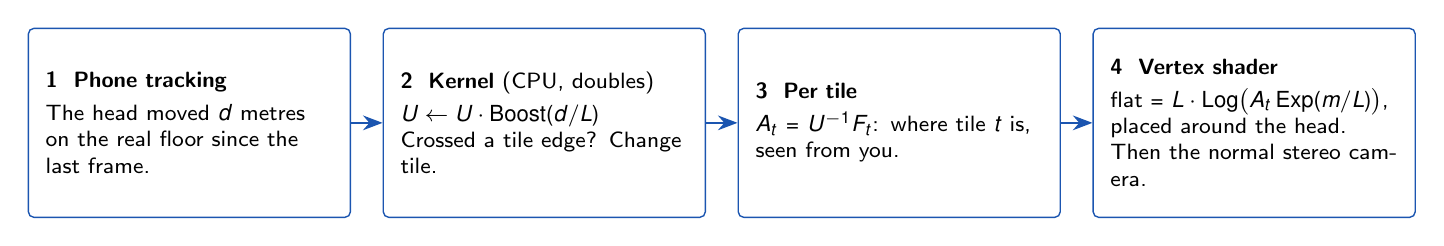
\begin{tikzpicture}[>=Stealth,
  box/.style={draw=accD,line width=0.5pt,rounded corners=2pt,text width=36.5mm,minimum height=24mm,inner sep=2.2mm,align=left,font=\footnotesize}]
\node[box] (a) {\textbf{1\ \ Phone tracking}\\[0.8mm] The head moved $d$ metres on the real floor since the last frame.};
\node[box,right=4mm of a] (b) {\textbf{2\ \ Kernel} (CPU, doubles)\\[0.8mm] $U \leftarrow U\cdot\mathrm{Boost}(d/L)$\\ Crossed a tile edge? Change tile.};
\node[box,right=4mm of b] (c) {\textbf{3\ \ Per tile}\\[0.8mm] $A_t = U^{-1}F_t$: where tile $t$ is, seen from you.};
\node[box,right=4mm of c] (d) {\textbf{4\ \ Vertex shader}\\[0.8mm] $\text{flat} = L\cdot\mathrm{Log}\big(A_t\,\mathrm{Exp}(m/L)\big)$, placed around the head. Then the normal stereo camera.};
\draw[->,line width=0.9pt,accD] (a)--(b);
\draw[->,line width=0.9pt,accD] (b)--(c);
\draw[->,line width=0.9pt,accD] (c)--(d);
\end{tikzpicture}
\end{center}

\Sub{Where a point lives}

One number picks the geometry: $\kappa=-1$ hyperbolic, $0$ flat, $+1$ spherical. Only the floor is curved; height stays ordinary ($\Hyp\times\R$ and $\Sph\times\R$). A point of the hyperbolic floor is a 3-vector $p=(x,z,w)$ on the \textbf{hyperboloid}
\[
x^2+z^2-w^2=-1,\quad w>0,\qquad \text{start point } o=(0,0,1),\qquad \langle a,b\rangle=a_xb_x+a_zb_z-a_wb_w .
\]
The sphere is the same with the sign flipped: $x^2+z^2+w^2=1$. We use this model because every motion of the floor (a walk, a turn) is then a $3\times3$ matrix, and one motion after another is a matrix product, exactly as rotations work for a sphere. The Poincar\'e disc is used only to draw the map.

Lengths inside the kernel are in units of $L$, the curvature radius (curvature $K=-1/L^2$); multiplying by $L$ gives metres.

\begin{center}\small
\begin{tabular}{@{}lll@{}}
\toprule
 & \textbf{Hyperbolic} ($\kappa=-1$) & \textbf{Sphere} ($\kappa=+1$)\\
\midrule
Distance between $p$ and $q$ & $\cosh d=-\langle p,q\rangle$ & $\cos d=p\cdot q$\\
$\mathrm{Exp}$: flat vector $t$, $r=|t|$, to a point & $\big(\sinh r\cdot t/r,\ \cosh r\big)$ & $\big(\sin r\cdot t/r,\ \cos r\big)$\\
$\mathrm{Log}$: point $p$ to a flat vector & $\operatorname{asinh}(|p_{xz}|)\cdot p_{xz}/|p_{xz}|$ & $\operatorname{acos}(p_w)\cdot p_{xz}/|p_{xz}|$\\
Undo a motion $M$ & $M^{-1}=\eta M^{\mathsf T}\eta,\ \ \eta=\mathrm{diag}(1,1,-1)$ & $M^{-1}=M^{\mathsf T}$\\
\bottomrule
\end{tabular}
\end{center}

\Sub{Step in: the walker's pose}

The pose is a pair (tile, $U$): which tile you are in, and a $3\times3$ matrix $U$ that says where you are in it and which way you face. Each frame the phone gives the head's floor displacement $d$ (metres), and
\[
U\ \leftarrow\ U\cdot\mathrm{Boost}(d/L),\qquad
\mathrm{Boost}(\Delta)=\exp\!\begin{pmatrix}0&0&\Delta_x\\0&0&\Delta_z\\-\kappa\Delta_x&-\kappa\Delta_z&0\end{pmatrix}
=\begin{pmatrix}1+(c-1)u_x^2&(c-1)u_xu_z&s\,u_x\\(c-1)u_xu_z&1+(c-1)u_z^2&s\,u_z\\s\,u_x&s\,u_z&c\end{pmatrix}
\]
with $u=\Delta/|\Delta|$, $c=\cosh|\Delta|$, $s=\sinh|\Delta|$ (written out for $\kappa=-1$; the sphere uses $\cos$, $\sin$ and a minus sign on the last row; at $\kappa=0$ it is a plain translation). This is a \textbf{Lorentz boost}, the matrix of special relativity, with the two floor axes as space and $w$ as time.

\begin{itemize}
\item A step larger than 0.2\,m in one frame, or a frame where tracking is not Normal, counts as no step.
\item $U$ is put back onto the group every frame (Gram--Schmidt with respect to $\eta$), so rounding never builds up.
\item The kernel is one class, \code{HolonomyWalkerKernel}: flat, hyperbolic \{4,5\} or \{4,6\}, or the sphere, by configuration.
\end{itemize}

\Sub{Why the path matters (holonomy)}

Take the instruction ``walk $s$, turn left $90^\circ$'': $g=\mathrm{Boost}(s/L)\cdot\mathrm{Rot}(90^\circ)$. In each geometry $g$ is a rotation by an angle $\phi$ about some fixed point, and the walk closes after $n$ sides when $\phi=360^\circ/n$:

\[
\cos\frac{\phi}{2}=\frac{\cosh(s/2L)}{\sqrt2}\ \ \text{(hyperbolic)},\qquad\qquad
\cos\frac{\phi}{2}=\frac{\cos(s/2R)}{\sqrt2}\ \ \text{(sphere)}.
\]
\begin{minipage}[c]{0.47\textwidth}
\small
\begin{tabular}{@{}cll@{}}
\toprule
\textbf{Sides to close} & \textbf{Geometry} & \textbf{Side length}\\
\midrule
3 & sphere & $s/R=\pi/2=1.5708$\\
4 & flat & any\\
5 & hyperbolic \{4,5\} & $s/L=1.0613$\\
6 & hyperbolic \{4,6\} & $s/L=1.3170$\\
never & hyperbolic & $s/L\ge1.7627$\\
\bottomrule
\end{tabular}
\end{minipage}\hfill
\begin{minipage}[c]{0.50\textwidth}
\centering
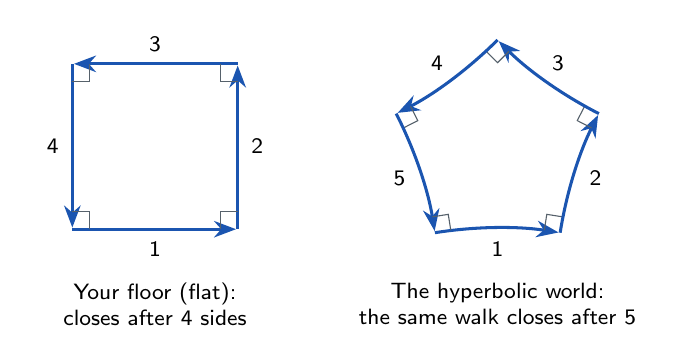
\begin{tikzpicture}[>=Stealth]
% the square on the floor
\begin{scope}
\foreach \a/\b/\c/\d in {0/0/2.1/0, 2.1/0/2.1/2.1, 2.1/2.1/0/2.1, 0/2.1/0/0}
  \draw[->,line width=1.1pt,accD,shorten >=0.6pt] (\a,\b)--(\c,\d);
\foreach \x/\y/\r in {0/0/0, 2.1/0/90, 2.1/2.1/180, 0/2.1/270}
  \draw[mute,line width=0.4pt,shift={(\x,\y)},rotate=\r] (0.22,0)--(0.22,0.22)--(0,0.22);
\node[font=\footnotesize] at (1.05,-0.25) {1};
\node[font=\footnotesize] at (2.35,1.05) {2};
\node[font=\footnotesize] at (1.05,2.35) {3};
\node[font=\footnotesize] at (-0.25,1.05) {4};
\node[font=\footnotesize,align=center,text width=30mm] at (1.05,-0.95) {Your floor (flat):\\closes after 4 sides};
\end{scope}
% the right-angled pentagon in the Poincare disc (drawn enlarged)
\begin{scope}[shift={(5.4,1.05)},scale=3.4]
\foreach \k/\lab in {0/1,1/2,2/3,3/4,4/5} {
  \begin{scope}[rotate=72*\k-90]
  \draw[->,line width=1.1pt,accD,shorten >=0.6pt] (0.321965,-0.233920) arc[start angle=189,end angle=171,radius=1.49538];
  \draw[mute,line width=0.4pt] (0.321965,0.233920) ++(171:0.06) -- ++(261:0.06) -- ++(351:0.06);
  \end{scope}
  \node[font=\footnotesize] at (72*\k-90:0.385) {\lab};
}
\end{scope}
\node[font=\footnotesize,align=center,text width=40mm] at (5.4,-0.95) {The hyperbolic world:\\the same walk closes after 5};
\end{tikzpicture}
\end{minipage}

\textbf{What you feel.} Your floor is flat, so four sides bring your body back to the same spot. In the world they do not: after one lap you are one side-length away and turned $90^\circ$, so you stand in the next room. Five laps bring the first room back. In general, carrying a direction round a closed loop turns it by (area of the loop)$/L^2$ (Gauss--Bonnet).

\textbf{Loop-fit rule.} We choose $L$ so that the square that fits \emph{your} room is the five-corner square. From the scan's free rectangle $W_f\times D_f$: $s=\mathrm{clamp}(\min(W_f,D_f)-0.4\,\text{m},\ 1.0,\ 3.2)$, then $L=s/1.0613$ (five rooms per corner), $L=s/1.3170$ (six) or $R=2s/\pi$ (planet). Example: $s=2.0$\,m gives $L=1.88$\,m.

\Sub{The world: tiles with exact addresses}

The hyperbolic floor is cut into square tiles, five at every corner: the \{4,5\} tiling. In units of $L$: centre spacing 1.0613 (its $\cosh$ is the golden ratio $\varphi$), corner angle $72^\circ$, corner distance 0.8425, area $2\pi/5$. The spacing is the same 1.0613 as above: ``rooms per corner'' and ``sides to close'' are one number.

\begin{itemize}
\item \textbf{Room to spare.} Tiles at 0, 1, 2, \dots\ steps away: 1, 4, 12, 28, 64, 148, 340, 780. That is about $\times2.3$ per ring; flat squares give 1, 4, 8, 12, 16.
\item \textbf{Exact ids.} Stepping through edge $k$ is the matrix $S_k=R^kTH$, with $R$ a quarter turn, $H=\mathrm{diag}(-1,-1,1)$ and
$T=\left(\begin{smallmatrix}\varphi&0&\sqrt\varphi\\0&1&0\\\sqrt\varphi&0&\varphi\end{smallmatrix}\right)$.
Every entry is $u+v\varphi$ with whole numbers $u,v$, so a tile centre is $(\sqrt\varphi\,X,\sqrt\varphi\,Y,W)$ with $X,Y,W\in\mathbb{Z}[\varphi]$: \textbf{six integers}, with the check $\varphi(X^2+Y^2)-W^2=-1$. Because $\varphi^2=\varphi+1$, a neighbour step needs additions only.
\item \textbf{What that buys.} ``Which room am I in'' has no rounding error, ever. Walk five rooms round a corner and the id is exactly the first one again. A tile's content is a hash of its id, so a room is the same each time you return and nothing is stored. 64-bit integers are exact out to 42 straight tile steps.
\item \textbf{Staying accurate.} Hyperboloid coordinates grow like $e^{d}$. So when you cross edge $i$ the kernel does $U\leftarrow G_i^{-1}U$ and moves to the neighbour: $U$ only ever describes a place inside one tile and stays small.
\end{itemize}

\Sub{Draw out: the warp}

On the CPU, for each drawn tile $t$: $A_t=U^{-1}F_t$ (in doubles, cast to float last). In the vertex shader (\code{AtlasWarp.hlsl}), for each vertex $m$, given in metres in its tile's own flat chart:
\[
p=A_t\cdot\mathrm{Exp}(m_{xz}/L),\qquad t=L\cdot\mathrm{Log}(p),\qquad
\text{world position}=(\text{head}_x+t_x,\ \ m_y,\ \ \text{head}_z+t_z).
\]
\begin{itemize}
\item \textbf{Exact:} the distance and the direction of every point from your head. It is the map projection called azimuthal equidistant, centred on you. Rays from the head are straight in the picture, so what you see is what an eye in $\Hyp\times\R$ would see.
\item \textbf{Shrunk:} sideways lengths at distance $d$ are drawn at scale $(d/L)/\sinh(d/L)$: 0.85 at one unit, 0.30 at three. That is correct, not an error. Things fall away faster than in a flat room, which is how so many rooms fit in view.
\item \textbf{Stereo:} the warp is centred on the head, not on each eye; the two eye cameras then give correct depth.
\item \textbf{Fog for free:} flat distance from the head divided by $L$ is the true geodesic distance. Fog starts at $\rho-1$ and is solid at $\rho=3$ units. A tile is drawn when its centre is within $\rho+0.8425$: at most 71 tiles.
\item \textbf{Seamless tiles:} each tile mesh is a grid in the Klein model, where straight lines are geodesics, so neighbours share their edge exactly. Grid point $k$ goes to the chart point $L\cdot\operatorname{atanh}(|k|)\cdot k/|k|$.
\item \textbf{Your room:} the scanned room and its furniture sit in tile zero and pass through the same warp. At $\kappa=0$ the warp is the identity, so the room matches the real one. Curvature is ramped in over 4\,s, and only while you stand still (head speed at most 0.1\,m/s).
\end{itemize}

\begin{asked}
\Q{Why the hyperboloid and not the Poincar\'e disc?} Motions are plain matrices and composing them is a matrix product, as with rotations of a sphere; it is also numerically stable. The disc is only our map picture: $\rho=\tanh(r/2)$.
\Q{What is distorted?} Nothing along a ray from your head. Sideways lengths shrink with distance, exactly as hyperbolic space looks from inside.
\Q{How do you avoid drift?} Integer tile ids, a pose kept inside the current tile, re-orthonormalising every frame, doubles on the CPU and one cast to float at the end.
\Q{How do you know it is right?} Unit tests on Exp and Log, the holonomy, the closing of the five-sided lap and the tile ids; a recorded five-sided lap closes to under 0.25\,m in the end-to-end test. The pass mark for the shader is 1\,mm from the CPU reference out to three units.
\end{asked}

% ====================================================================================================
\Sec{Rendering and performance}

\Sub{One frame, in order}

\begin{center}
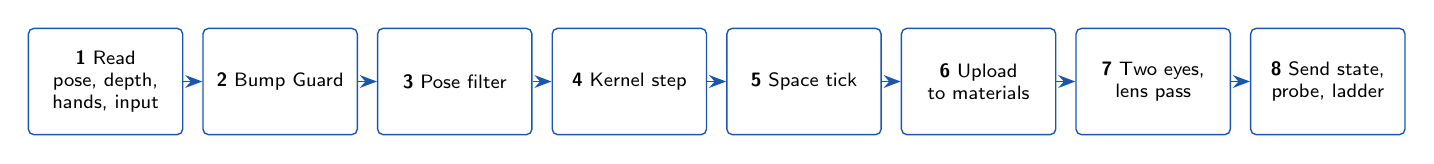
\begin{tikzpicture}[>=Stealth,
  st/.style={draw=accD,line width=0.5pt,rounded corners=2pt,text width=17.0mm,minimum height=13.5mm,inner sep=1.3mm,align=center,font=\scriptsize}]
\node[st] (a) {\textbf{1} Read pose, depth, hands, input};
\node[st,right=2.4mm of a] (b) {\textbf{2} Bump Guard};
\node[st,right=2.4mm of b] (c) {\textbf{3} Pose filter};
\node[st,right=2.4mm of c] (d) {\textbf{4} Kernel step};
\node[st,right=2.4mm of d] (e) {\textbf{5} Space tick};
\node[st,right=2.4mm of e] (f) {\textbf{6} Upload to materials};
\node[st,right=2.4mm of f] (g) {\textbf{7} Two eyes, lens pass};
\node[st,right=2.4mm of g] (h) {\textbf{8} Send state, probe, ladder};
\foreach \x/\y in {a/b,b/c,c/d,d/e,e/f,f/g,g/h} \draw[->,line width=0.7pt,accD] (\x)--(\y);
\end{tikzpicture}
\end{center}

Steps 1 to 7 never wait for the network, and Bump Guard runs before anything that could fail. A space is a module (\code{ISpaceModule}: configure, enter, tick, exit) hosted by one scene, \code{SpaceLab}, with a 0.25\,s fade between spaces. Everything is built in code at boot.

\Sub{Stereo and the lens}

\begin{itemize}
\item Two eye cameras 64\,mm apart, each drawing into its own texture: $1118\times1032$\,px with $4\times$ MSAA. No XR plug-in.
\item One full-screen pass then bends both pictures for the lenses: $r'=r\,(1+K_1r^2+K_2r^4)$. The lens numbers are Cardboard-class placeholders, tunable live from the Console.
\item Optional gyro prediction (off by default) turns the eyes up to 40\,ms ahead. The kernel and Bump Guard never see it.
\end{itemize}

\Sub{One shader, a diagram look}

Every surface uses \code{Atlas/Surface}: one pass, one variant, no keywords.
\begin{itemize}
\item Colour from a small palette, shade baked into vertex colours, \textbf{no lighting from normals}; grid and edge lines from screen-space derivatives; fog to the horizon colour. The warp is its vertex stage; the portal clip and the sight-line gates are in its fragment stage.
\item No lights, shadows, HDR or post-processing. One material layout and pooled materials, so the SRP Batcher can batch everything.
\item Why flat: lightmaps and normals cannot follow warped geometry, and a line drawing of a curved world reads better than a lit one.
\end{itemize}

\Sub{Budgets and the thermal ladder}

Targets per frame: at most 300 draw calls and 500,000 triangles for both eyes. Curved Walk is the heaviest space (240 draw calls, 370,000 triangles); Home is 80 and 250,000.

\begin{center}\small
\begin{tabular}{@{}lcccccc@{}}
\toprule
\textbf{Tier} & \textbf{Render scale} & \textbf{MSAA} & \textbf{Draw radius $\rho$} & \textbf{Glued copies} & \textbf{Furniture} & \textbf{Frames per second}\\
\midrule
Nominal & 0.8 & $4\times$ & 3 & $5\times5$ & full & 60\\
Fair & 0.7 & $4\times$ & 3 & $5\times5$ & light & 60\\
Serious & 0.6 & $2\times$ & 2 & $3\times3$ & light & 60\\
Critical & 0.6 & off & 2 & $3\times3$ & light & 30\\
\bottomrule
\end{tabular}
\end{center}

The ladder steps down one tier at a time, at most once per 20\,s, when the phone's thermal state rises or the GPU time's 95th percentile passes 9\,ms, then 12\,ms. Quality drops before the frame rate does; the floor is 30.

\Status{No frame rate, frame time or thermal figure has been measured on a phone yet; the target is 60 frames a second. Measured elsewhere: 0 bytes of managed allocation over 100 frames in S0 to S6 (headless), and a tile-crossing frame's kernel and upload at 0.94\,ms at the 95th percentile (Editor). Motion-to-photon is estimated at 55 to 95\,ms, not measured. The app carries its own performance tour to produce the real numbers.}

\begin{asked}
\Q{Does it hold 30 frames a second?} It is built for 60, with a ladder that gives up quality before frame rate and a floor of 30. Say the number only once it is measured on the phone.
\Q{How is stereo made?} Two cameras into two textures, then one lens pass. We wrote the rig ourselves.
\Q{Why does it look like a diagram?} By choice: one cheap shader that still works when the geometry is warped.
\end{asked}


% ====================================================================================================
\Sec{The other spaces}

\Sub{S1 Glued: torus, Klein bottle, 3-torus}
\begin{itemize}
\item \textbf{Maths.} A torus is the flat floor with points identified under two translations $A$ and $B$. In the Klein bottle $B$ also mirrors left and right. The 3-torus adds a vertical translation $C$ of 2.6\,m.
\item \textbf{Built as a lattice of copies,} fixed to the floor: copy (col, row, layer) is $A^{col}B^{row}C^{layer}$, a mirror flag plus a translation. We draw $5\times5$ copies of the cell (3, 5 or 7 by thermal tier; 27 for the 3-torus). In the Klein bottle the odd rows are drawn mirrored.
\item \textbf{Nobody is teleported.} The walker is never moved; a copy of the walker, with their hands, stands in every other cell. So you see your own back, and in the Klein bottle your copy waves the other hand.
\end{itemize}

\Sub{S3 Aligned Cells: the hyperbolic world from flat pieces}
\begin{itemize}
\item The real floor is cut into flat square cells of side $g$ (about 1.5\,m). Each edge you cross is one step in the same \{4,5\} tile graph as Curved Walk. Four cells meet at a post on the floor, but five tiles meet there in the world, so one walk round a post ends in a fifth room.
\item \textbf{All the curvature sits at the posts.} The angle round a post is $5\times90^\circ=450^\circ$, a curvature of $-\pi/2$ per post, and $4\times(-\pi/2)/5=-2\pi/5$ per tile: the same as the smooth tile. The equivalent radius is $0.892\,g$.
\item \textbf{Sight-line gates.} What a cell shows depends on which way round the posts you look at it. The shader clips each pixel by the sign of $(\text{post}-\text{eye})\times(\text{pixel}-\text{eye})$, with up to four gates, per eye, and no stencil. At most 57 cell instances are drawn.
\item Every piece is flat, so the picture matches the real room and the furniture stays where it really is. It is the fallback way to walk the hyperbolic world.
\end{itemize}

\Sub{S4 Small Planet: the sphere}
\begin{itemize}
\item The \{4,3\} tiling: the six faces of a cube blown onto a sphere, all always drawn. The same kernel with $\kappa=+1$: $U\leftarrow U\cdot\mathrm{Boost}(d/R)$ with $\cos$ and $\sin$.
\item $R=\max(2s/\pi,\ 2.0\,\text{m})$, so the planet is at least 12.6\,m round. Three right-angle turns close a triangle when a side is a quarter of the way round: 3.14\,m at the default $R=2.0$\,m. In a smaller room, lower \code{planet.R} so that the lap square closes it.
\item Fog runs from $0.5\pi$ to $0.8\pi$ radians, and pixels beyond 2.6 radians are discarded, because the log map smears near the point opposite you.
\end{itemize}

\Sub{S5 Impossible Rooms: portals}
\begin{itemize}
\item The rooms overlap on the same real floor, so every portal's transform is the identity. \textbf{Nobody is teleported}, and the real floor stays under your feet. A 1\,m booth holds a hall as large as the whole floor; a corridor with four right turns ends in a different room.
\item \textbf{Which room you see is chosen per pixel.} Each visible doorway takes a stencil value (15 at most). A mask marks the doorway and resets depth; the room behind is drawn with the stencil test and a clip plane. There is no extra camera and no render texture, one level deep.
\item \textbf{Crossing.} When the head passes the doorway's plane, the current room swaps. The layout is generated from the free rectangle (doors 0.9\,m wide, 2 to 6 rooms).
\end{itemize}

\Sub{S6 Slicer: four dimensions}
\begin{itemize}
\item A 4D body is a mesh of tetrahedra with 4D vertices: the tesseract (48 tetrahedra), the 5-cell, 16-cell and 24-cell, a ball, and tubes of 18,000.
\item \textbf{The cut.} Every frame, on the CPU in a Burst job, each tetrahedron is cut by the hyperplane $n\cdot x=w_0$. With $f_i=n\cdot x_i-w_0$ at each vertex, every edge whose ends have opposite signs gives the point
$x_i+\frac{f_i}{f_i-f_j}(x_j-x_i)$. Three such points make a triangle, four a quadrilateral.
\item \textbf{Controls.} Walking along a lane on the floor moves the cut along $w$. The body turns in the XW, YW and ZW planes. Beside the slice is the shadow, $xyz\cdot f/(f-w)$ with $f=2$.
\item \textbf{Check.} The unit tesseract cut by $x+y+z+w=c$ is a regular tetrahedron of area 0.8660 at $c=0.5$ and a regular octahedron of area 6.9282 at $c=2$.
\end{itemize}

\begin{asked}
\Q{Do the portals teleport you?} No. All the rooms share one floor; a stencil mask picks the room for each pixel.
\Q{Torus or Klein bottle: what changes?} The same lattice. The Klein bottle mirrors every other row, so your copy waves the other hand.
\Q{Where is the curvature in Aligned Cells?} At the posts: $450^\circ$ round each one, which adds up to the same $-2\pi/5$ per tile as the smooth world.
\Q{Is the 4D real?} Yes. Real 4D tetrahedra are cut by a hyperplane every frame, checked against known slice areas.
\end{asked}


% ====================================================================================================
\Sec{Safety: Bump Guard}\label{sec:safety}

The headset view is generated, and in a curved space the virtual walls are not where the real walls are. So safety cannot come from the picture. \textbf{Bump Guard reads only the physical layer}: the real head pose, the scan's distance field and the live LiDAR depth image. No space feeds it anything, and it runs first in every frame.

\Sub{Every frame}

\begin{enumerate}
\item \textbf{New obstacles from live depth.} The depth image is sampled. A return that is 0.10 to 2.0\,m above the floor and more than 0.30\,m nearer than the scan predicts marks a 5\,cm cell: a person who walked in, a moved chair. The cell clears when three images see through it, or after 30\,s.
\item \textbf{Velocity.} The head's movement over the last 0.2\,s.
\item \textbf{Clearance.} $\mathrm{clear}(p)$ is the smaller of the scan's distance field and the distance to the nearest marked cell. \emph{now} is the clearance at the head; \emph{path}($T$) is the smallest clearance on the straight line of the next $T$ seconds.
\item \textbf{Two levels.} WARN when now $<0.30$\,m or path(0.8\,s) $<0.05$\,m. STRONG when now $<0.20$\,m or path(0.4\,s) $<0.05$\,m.
\item \textbf{Hysteresis.} A level rises at once and falls only after the thresholds plus 0.05\,m have held for 0.3\,s, so the cue does not flicker.
\item \textbf{Tracking lost.} It falls back to depth alone (the nearest return in seven $10^\circ$ sectors) and says ``stand still'' after 0.5\,s.
\end{enumerate}

\begin{itemize}
\item \textbf{The cue} is fixed to the head and never warped. WARN: an amber chevron on the hazard's side, a tick, two haptic pulses a second. STRONG: a larger red chevron, a tone, six pulses a second. There is no off switch.
\item \textbf{Independence.} The safety assembly may not reference the link or the telemetry; a test enforces it. A Wi-Fi drop cannot touch it.
\item \textbf{Limits.} Live depth covers only where the head looks (0.3 to 5\,m), and nothing lower than 0.10\,m is covered.
\end{itemize}

\Status{Proven headless, on synthetic depth and recorded walks: 20 scripted approaches warn at least 0.6\,s before contact; ten wall approaches at 0.5 to 1.0\,m/s lead by 0.85 to 0.93\,s; a recorded lap gives no STRONG cue and two corner WARNs. The per-space run still skips the three curved spaces (S2 to S4). The on-phone checks (20 of 20 real approaches, with a spotter) are not recorded yet. The cost target is 0.3\,ms a frame.}

\begin{asked}
\Q{How do you stop a walker hitting a wall?} We predict the head's path 0.4 and 0.8\,s ahead against the real obstacles, and a chevron, a sound and a haptic pulse point at the hazard.
\Q{Virtual walls are not real walls. Why does it work?} Bump Guard ignores the virtual world. It uses the real pose and the real scan only.
\Q{What about a person who walks in?} Live depth marks anything more than 0.30\,m nearer than the scan predicts, where the head is looking.
\end{asked}


% ====================================================================================================
\Sec{Tracked hands and input}

The walker cannot see their own hands in a generated view. Tracked hands draw each hand where it is felt, and let a fingertip press and a pinch select. Gaze dwell (0.7\,s), the headset lever and the gamepad always work as well.

\Sub{From a camera frame to a hand in the room}

\begin{enumerate}
\item \textbf{Detect.} Apple Vision's hand-pose request (\code{VNDetectHumanHandPoseRequest}) runs in our Swift plugin on the camera frame ARKit already has: 21 joints per hand as picture points with a confidence each, up to two hands, 30 times a second. No image is stored.
\item \textbf{Depth.} LiDAR depth is sampled at every joint (the median of $3\times3$ pixels) and at up to 64 points across the palm.
\item \textbf{Palm.} A plane is fitted to the palm samples by least squares (outliers over 2.5\,cm dropped). It is valid from 0.32 to 0.90\,m; nearer than that, the distance comes from the hand's known size.
\item \textbf{Fingers, bone by bone.} Each joint lies on its camera ray at one bone's length from its parent, which gives two candidates. The eight chains of a finger are scored by anatomy, by LiDAR and by the last frame. LiDAR never places a fingertip; it only chooses.
\item \textbf{Hand size.} Bone lengths and scale (0.80 to 1.25) are learnt per walker from 30 square-on sightings.
\item \textbf{Frames.} Pixel, to the camera at capture time, to the ARKit session, to the room. A head turn after the capture therefore does not move the hand.
\item \textbf{Smooth and predict.} A One-Euro filter (palm 1.5\,Hz, fingers 2.5\,Hz); the palm is predicted up to 50\,ms ahead; a result older than 0.2\,s is dropped. A lost hand holds for 0.25\,s, then fades.
\item \textbf{Draw.} A 790-triangle hand mesh, skinned on the CPU, that fades at the edge of the camera's view.
\end{enumerate}

\Sub{Gestures}

\begin{itemize}
\item \textbf{Pinch selects what you look at.} The measure is the thumb-tip to index-tip gap divided by the palm width. It closes under 0.25 on three detections in a row and opens over 0.40. It is ignored in a hand's first 0.3\,s, above 1\,m/s, and within 0.4\,s of the last pinch. It fires the target under the gaze at once, with no dwell.
\item \textbf{Fingertip press.} The index fingertip hovers within 8\,cm of a target's face, arms 2.5\,cm in front of it, and presses when it crosses a plane 1\,cm behind the face while moving more in than across. In a hands session the targets sit 0.48\,m from the camera and $25^\circ$ below the horizon, so looking at them brings the hands into view.
\item \textbf{Touch ring.} Reaching for a scanned wall or table shows a ring under the fingertip from 8\,cm; at 1.5\,cm it is contact, with a tap sound. The real surface is there to be felt.
\end{itemize}

\Sub{With the rest of the app}

\begin{itemize}
\item \textbf{Bump Guard.} A box round each hand is masked out of live depth, only at the hand's own depth and never beyond 0.80\,m. The scanned map is never masked. While a warning shows, the hands fade and fire nothing.
\item \textbf{Heat.} 30\,Hz normally, 15\,Hz when the phone is warm, stopped when it is hot; 5\,Hz when no hand has been seen for 20\,s.
\item \textbf{Field of view.} The camera sees about $72^\circ\times44^\circ$; each eye sees about $100^\circ\times96^\circ$. Hands are tracked only inside the camera's view.
\item \textbf{Glued rooms.} Every copy of the walker carries the walker's hands, in the same mesh, with no extra draw call.
\item \textbf{Demo tip.} First hold an open hand square to the camera for a second or two. Until the hand's size is learnt, a press nearer than 0.32\,m may not fire.
\end{itemize}

\Status{Built and merged; 322 hands tests, 117 input tests and 12 end-to-end tests pass headless. Not yet run in the Editor or on a phone, and \code{hands.enabled} is off by default. Hands sessions stay standing until the walking check with a spotter has passed. Fingertip accuracy and latency are not measured: the expected result age is 70 to 110\,ms, and a headless test with synthetic noise holds the fingertip within 30\,mm at the 95th percentile.}

\begin{asked}
\Q{Why Apple Vision and not MediaPipe?} Vision reads ARKit's own frame, so it never fights the AR session for the camera, and it needs no package or model file. MediaPipe is the named fallback behind the same interface; it is not built.
\Q{Vision gives 2D joints. Where does 3D come from?} LiDAR depth for the palm, then bone lengths along each joint's camera ray for the fingers.
\Q{Do raised hands trip the collision warning?} They are masked from live depth at the hand's own depth. The cost we accept: a hand held ahead hides what is right behind it.
\end{asked}


% ====================================================================================================
\Sec{The Forge: furniture from photos, with TripoSG}\label{sec:forge}

Every scanned object gets a real-looking mesh, generated on the Station from its photos. Until it arrives, the phone shows a simple first shape.

\Sub{How TripoSG works}

The model is from the paper ``TripoSG: High-Fidelity 3D Shape Synthesis using Large-Scale Rectified Flow Models'' (arXiv 2502.06608, February 2025; VAST, The Chinese University of Hong Kong, The University of Texas at Austin and Shanghai AI Laboratory).

\begin{itemize}
\item \textbf{A shape is a signed distance field (SDF):} for any point, the distance to the surface, negative inside. The surface is where it is zero. This holds finer geometry than an inside/outside grid.
\item \textbf{A VAE compresses the shape.} A transformer packs 20,480 surface points with their normals into latent tokens (up to 2,048 tokens of 64 channels), trained with SDF, surface-normal and eikonal losses.
\item \textbf{The generator is a rectified-flow transformer} of about 1.5 billion parameters (the public weights). Rectified flow learns the velocity along a straight path from noise to a shape's latent; generating is integrating that path in $N$ steps (we use 50).
\item \textbf{The photo steers it} through cross-attention in every block, on DINOv2 image features of a $224\times224$ input, with classifier-free guidance.
\item \textbf{A mesh comes out} by decoding the SDF on a grid (512 cells a side) and extracting its zero surface (marching cubes; the package \code{diso} does this on the GPU).
\item \textbf{Training:} 2 million curated objects. \textbf{Output:} shape only, with no colour and no real-world size. Our clean-up adds both.
\end{itemize}

\Sub{Our pipeline}

\begin{enumerate}
\item \textbf{Capture} (phone, during the scan). Up to 96 key frames are kept. Each object gets 1 to 3 views at least $30^\circ$ apart, taken from 0.6 to 3.0\,m. A crop is the object's projected box plus 12\,\% a side, squared, at most 768\,px.
\item \textbf{Upload.} The crops, with the box size, yaw and category, the cameras, and a 256-byte height profile of the object from the LiDAR scan.
\item \textbf{Matte.} The background is removed (\code{rembg}); the object is set on white, square, with a 10\,\% margin.
\item \textbf{Generate.} TripoSG: 50 steps, guidance 7.0, fixed seed, half precision, 90\,s time-out.
\item \textbf{Clean-up.} Weld and decimate; turn the mesh to the pose that best fits the scanned profile; scale it to the scanned box; regrid so no edge is longer than 0.25\,m (the warp bends vertices, so long edges would stay straight); colour each face from the photos; bake shade and ambient occlusion into vertex colours; make a light copy.
\item \textbf{Validate.} One mesh, no texture, 1,500 to 15,000 triangles, at most 2\,MB, within 10\,\% of the scanned box. The room's budget is 32 meshes and 120,000 triangles, shared by surface area.
\item \textbf{Deliver.} A GLB file named by its SHA-256. The phone hears of it through the Hub (or polls every 2\,s), checks the hash and the contract off the main thread, and fades the mesh in over 0.3\,s.
\end{enumerate}

\begin{itemize}
\item \textbf{First shapes.} At once, with or without the Forge: a template fitted to the scan (chair, couch, bed), a shape cut from the scan, or a box; at most 1,500 triangles. It stays if the Forge is away or a job fails.
\item \textbf{Self-check.} Each result is scored against the LiDAR profile. A poor fit tries the next photo, at most three generations per object, and the best one is published.
\end{itemize}

\Status{TripoSG has run on an RTX 4060 laptop (4 October): 87\,s per object at 50 steps, against a 60\,s target. No run is recorded on the Station's RTX 5070. A commit of 4 October notes three phone scans that sent the Forge no photos, so check the phone-to-Forge path end to end before calling it live. The tests use a procedural stand-in for the generator.}

\begin{asked}
\Q{Why TripoSG?} MIT licence, one photo in, and it fits an 8\,GB graphics card. TRELLIS needs 16\,GB and SAM 3D Objects 32\,GB.
\Q{Why not on the phone?} 1.5 billion parameters, about 8\,GB of weights and a CUDA-only decoder. The phone shows first shapes and downloads a file of at most 2\,MB.
\Q{What if the mesh is wrong?} It is scored against the LiDAR profile and must pass the contract; if it fails, the first shape stays.
\Q{Licences?} TripoSG's code and weights are MIT. The \code{diso} decoder is CC BY-NC 4.0: fine for a demo, open for commercial use.
\end{asked}

% ====================================================================================================
\Sec{The Station and the link}

The Station is the PC beside the walker. Four programs run on it.

\begin{center}\small
\begin{tabularx}{\textwidth}{@{}l l >{\raggedright\arraybackslash}X@{}}
\toprule
\textbf{Program} & \textbf{Built with} & \textbf{What it does}\\
\midrule
Hub & .NET 8 console; UDP 9050, HTTP 8080 & Ends the phone link, relays the phone's state to Spectators, sends parameters and operator commands to the phone, writes the session logs, serves the Console and the pairing page.\\
Console & a web page served by the Hub & Live state at 10\,Hz, a slider for every registered parameter, presets, and the operator commands: home, recentre, quality tier, STOP cue, demo lock, change space.\\
Spectator & Unity build for Windows & Redraws the walker's view from the relayed state with the same kernel and the same warp, beside the ``flat twin'' map (floor plan, or Poincar\'e disc in the curved spaces).\\
Forge & Python 3.11, FastAPI, port 8000 & Turns object photos into furniture meshes (section \ref{sec:forge}).\\
\bottomrule
\end{tabularx}
\end{center}

\begin{itemize}
\item \textbf{Transport.} LiteNetLib over UDP, on the Station's own router with no internet. Pairing is a QR code holding \code{atlas://<station-ip>:9050}; the phone camera opens it and the app connects.
\item \textbf{State.} One 202-byte message, 60 times a second. The Hub relays it unchanged and appends it to \code{state.bin}, so any walk can be replayed.
\item \textbf{One source for the bytes.} The Hub compiles the app's own link source files, so the phone and the Hub cannot disagree about a byte of the protocol.
\item \textbf{Clock and latency.} The Hub pings every client (eight times 50\,ms apart, then four times a second), keeps a clock offset per client, and reports link latency at p50, p95 and p99.
\item \textbf{Watchdog.} A client is \emph{degraded} after 500\,ms of silence and \emph{offline} after 3\,s. The Hub keeps the last value of every parameter and gives them back to a phone that reconnects.
\item \textbf{Live tuning.} A slider on the Console becomes a \code{ParamSet}; the phone clamps the value and answers with what it applied. A demo lock makes the phone ignore changes.
\item \textbf{Logs per session.} \code{state.bin}, \code{events.jsonl}, \code{perf.csv} (34 columns, one row a second), \code{phone.log}, \code{hub.log}. Motion logs are treated as health data and kept on an encrypted volume.
\item \textbf{ReplayPhone.} A small program that plays a recorded or synthetic walk into the Hub, so the Console and the Spectator can be developed and tested with no phone.
\end{itemize}

\begin{itemize}
\item \textbf{No video is sent.} The state carries the head pose, the space, the tile id (six 64-bit integers), the walker matrix (nine doubles) and a few floats. The Spectator redraws the view itself and never integrates motion on its own.
\item \textbf{Channels.} Control messages are reliable and ordered; the state is sequenced (a late one is dropped, never replayed). Clock sync is a four-timestamp exchange that keeps the sample with the smallest round trip; the target is 2\,ms at the 95th percentile.
\item \textbf{If Wi-Fi drops,} the walker notices nothing: the phone renders and decides everything, retries the link, and keeps writing its own telemetry.
\end{itemize}

\Status{The Hub's 42 tests and the Console's 59 pass, and a rehearsal runs the Hub, the Forge and ReplayPhone together. No run of the Spectator's Windows build is recorded, and clock sync is not measured over Wi-Fi.}

\begin{asked}
\Q{What does the Station do that the phone cannot?} It runs TripoSG on a GPU, shows the audience the walk, and lets an operator tune and stop it.
\Q{Why not stream video to the PC?} The state is 202 bytes; a stereo video stream would cost the phone heat and latency. The Spectator has the same kernel, so it can redraw exactly.
\end{asked}


% ====================================================================================================
\Sec{Use cases}

\Sub{Network Atlas (S7): why the internet fits hyperbolic space}
\begin{itemize}
\item \textbf{Model:} Krioukov et al., \emph{Hyperbolic Geometry of Complex Networks} (2010). 200 nodes are scattered in a hyperbolic disc of radius $R=10.5$, more densely towards the rim. Two nodes are linked when their hyperbolic distance $x$ is under $R$:
$\cosh x=\cosh r\cosh r'-\sinh r\sinh r'\cos\Delta\theta$. Out come a few big hubs near the centre and many small nodes at the rim, as in real networks.
\item \textbf{Greedy routing:} hand the packet to the neighbour nearest the target. No routing table, no map.
\item \textbf{Built:} a disc on the Console and the Spectator, and a floor map in the headset: a Poincar\'e disc up to 1.2\,m in radius ($\rho=\tanh(r/2)$). Looking at a node re-centres the map on it with the M\"obius move $z\mapsto(z-a)/(1-\bar az)$ over 0.6\,s. A walk-through version is written and unit-tested but not wired in.
\item \textbf{Measured,} offline, on the same 1,000 random pairs: routing by hyperbolic distance delivers 100\,\% (seed 7) and 99.7\,\% (seed 83); routing by distance in the flat picture delivers 71.8\,\% and 72.6\,\%.
\item \textbf{Say:} ``a network \emph{generated} by this model''. \textbf{Do not say:} ``the real internet'', ``greedy always works'' or ``flat space cannot route''.
\end{itemize}

\Sub{Lung: a breathing chest as a 4D object}
\begin{itemize}
\item \textbf{Data:} TCIA 4D-Lung, patient 101, CC BY 3.0 (Hugo et al. 2016): a CT scan in 10 breathing phases, with real contours of the lesion, lungs, heart, oesophagus, spinal cord and trachea. A Station pipeline turns it into a case package (254 tests).
\item \textbf{Time is the fourth axis.} Phase $k$ sits at $\tau=1.5\,\text{m}\cdot k/10$ and wraps round: $\R^3\times S^1$. A surface followed through the ten phases becomes a 4D tube (each triangle sweeps a prism, split into three tetrahedra: 18,000 in all), and the Slicer cuts it. A straight cut is one phase. The shadow is everywhere the tumour goes. A tilted cut reproduces the motion artefact of a moving scanner table, $\tan\theta=c/v$.
\item \textbf{The airway as a tree in hyperbolic tiles.} One generation is a turn tile plus a straight tile, and a branch's address is a word of lefts and rights. A tree doubles with every generation; so does the hyperbolic floor (about $\times2.3$ per ring), so every branch gets a full-size room. On a flat floor the branches would collide.
\item \textbf{Two Compasses.} At some forks the straight-line compass points down the wrong branch (8.7\,\% of forks in our tree); the geodesic one does not.
\end{itemize}

\Status{The lung's organs and lesion are real contours, but the airway tree is model-generated, not this patient's. The app holds only a synthetic placeholder case today; the real package and the 4D tube are not wired into the headset. It is an education and research visualisation, not for clinical use: claim no clinical benefit.}

\Sub{FieldFit}
A teaching demo of visual-field loss: Home seen through a $10^\circ$ tunnel, then a lens that squeezes $54^\circ$ back into view, done with a $512\times512$ lookup per eye in the final pass. The parts exist and are tested; it is not wired into the app.

\begin{asked}
\Q{Is the lung real patient data?} The lesion and the organs are real, public contours. The airway is generated by a model, and the app's bundled case is synthetic.
\Q{Does greedy routing always work?} No. It is measured, not guaranteed: 100\,\% and 99.7\,\% here against about 72\,\% in the flat picture.
\end{asked}


% ====================================================================================================
\Sec{How we know it works}

\begin{itemize}
\item \textbf{Logic lives in engine-free classes} (\code{BumpGuardCore}, \code{FrameLoopCore}, the kernel, the link), so it can be tested without Unity.
\item \textbf{The headless harness} (\code{tools/headless/verify.py}) compiles every assembly against the real Unity libraries for the phone, the Station and the Editor, and runs the engine-free tests on .NET 8. It exists because only one Mac can build to the phones. It cannot check shaders, scenes or a device.
\item \textbf{Counts,} last recorded runs: 1,995 headless tests and 2,114 in Unity's EditMode, none failing, with every shader compiled for Metal; then 42 for the Hub, 59 for the Console, 53 for the Forge. The hands and the Network Atlas came after and add several hundred more.
\item \textbf{Recorded walks} are replayed through the real frame loop: a recorded five-corner lap leaves tile zero and closes to under 0.25\,m.
\item \textbf{Gates:} G0 contracts frozen, G1 first light on the phone, G2 the curved-walk spike, G3 spaces in the Editor, G4 spaces on the phone at budget, G5 scan, Home and Bump Guard, G6 the Station link, G7 exit. Every headless line is proven; the device lines are still open.
\end{itemize}

\Sub{What is proven where}

As recorded in the repository on 4 October. Correct it with what you have seen since.

\begin{center}\small
\begin{tabularx}{\textwidth}{@{}>{\raggedright\arraybackslash}p{47mm} >{\raggedright\arraybackslash}p{39mm} >{\raggedright\arraybackslash}p{30mm} >{\raggedright\arraybackslash}X@{}}
\toprule
\textbf{Part} & \textbf{Headless tests} & \textbf{Unity Editor} & \textbf{On a phone}\\
\midrule
Kernel, tiling, warp & pass & pass, shaders compile & no curved walk recorded\\
Scan and room model & pass & pass & ran to the end; accuracy not measured\\
Bump Guard & pass; lead 0.85 to 0.93\,s & pass & not recorded\\
Glued, Aligned Cells, Small Planet, Impossible Rooms, Slicer & pass & pass & not recorded\\
Tracked hands & pass (322 tests) & not run & not run; off by default\\
Forge and TripoSG & pass, with a stand-in generator & & TripoSG ran on a laptop GPU (87\,s); no photos arrived from three phone scans\\
Station link and Console & pass (42 and 59) & & not recorded\\
Network Atlas & pass, one app test failing & not run & not run\\
Lung, FieldFit & the parts pass & the parts pass & not in the app\\
Frame rate & & & no figure yet\\
\bottomrule
\end{tabularx}
\end{center}

\Key{\textbf{Before you say it to a judge.}
\begin{itemize}
\item A frame rate: only once it is measured on the phone.
\item ``Any phone'': it needs an iPhone with LiDAR.
\item Hands, generated furniture and the lung in the headset: say ``built and tested off the device'' unless you have seen it live.
\item TripoSG's authors: VAST, The Chinese University of Hong Kong, UT Austin and Shanghai AI Laboratory.
\item The network result: ``in our generated network, 100\,\% against about 72\,\%''.
\end{itemize}}



\end{document}
